\documentclass[10pt,journal,compsoc]{IEEEtran}
\usepackage[nocompress]{cite}
\usepackage{graphicx}
\usepackage{subfigure}
\usepackage{url}
\usepackage{multirow}
\usepackage[ruled]{algorithm2e}
\usepackage{enumitem}

\newtheorem{theorem}{Theorem}[section]
\newtheorem{lemma}[theorem]{Lemma}
\newtheorem{observation}[theorem]{Observation}

\begin{document}

\title{Efficient Suffix Array Construction and Checking in External Memory}
%
%
% author names and IEEE memberships
% note positions of commas and nonbreaking spaces ( ~ ) LaTeX will not break
% a structure at a ~ so this keeps an author's name from being broken across
% two lines.
% use \thanks{} to gain access to the first footnote area
% a separate \thanks must be used for each paragraph as LaTeX2e's \thanks
% was not built to handle multiple paragraphs
%
%
%\IEEEcompsocitemizethanks is a special \thanks that produces the bulleted
% lists the Computer Society journals use for "first footnote" author
% affiliations. Use \IEEEcompsocthanksitem which works much like \item
% for each affiliation group. When not in compsoc mode,
% \IEEEcompsocitemizethanks becomes like \thanks and
% \IEEEcompsocthanksitem becomes a line break with idention. This
% facilitates dual compilation, although admittedly the differences in the
% desired content of \author between the different types of papers makes a
% one-size-fits-all approach a daunting prospect. For instance, compsoc 
% journal papers have the author affiliations above the "Manuscript
% received ..."  text while in non-compsoc journals this is reversed. Sigh.

\author{Yi~Wu,
        Ge~Nong,
        Wai~Hong~Chan,
        and~Bin~Lao
\IEEEcompsocitemizethanks{
\IEEEcompsocthanksitem Y. Wu, G. Nong (corresponding author) and B. Lao are with the Department of Computer Science, Sun Yat-sen University, Guangzhou 510275, China. E-mails: wu.yi.christian@gmail.com, issng@mail.sysu.edu.cn, Laobin@mail3.sysu.edu.cn.

\IEEEcompsocthanksitem Wai Hong Chan (corresponding author) is with the Department of Mathematics and Information Technology, The Education University of Hong Kong, Hong Kong. E-mail: waihchan@ied.edu.hk.
}}% <-this % stops a space
	
	

% note the % following the last \IEEEmembership and also \thanks - 
% these prevent an unwanted space from occurring between the last author name
% and the end of the author line. i.e., if you had this:
% 
% \author{....lastname \thanks{...} \thanks{...} }
%                     ^------------^------------^----Do not want these spaces!
%
% a space would be appended to the last name and could cause every name on that
% line to be shifted left slightly. This is one of those "LaTeX things". For
% instance, "\textbf{A} \textbf{B}" will typeset as "A B" not "AB". To get
% "AB" then you have to do: "\textbf{A}\textbf{B}"
% \thanks is no different in this regard, so shield the last } of each \thanks
% that ends a line with a % and do not let a space in before the next \thanks.
% Spaces after \IEEEmembership other than the last one are OK (and needed) as
% you are supposed to have spaces between the names. For what it is worth,
% this is a minor point as most people would not even notice if the said evil
% space somehow managed to creep in.



% The paper headers
%\markboth{Journal of \LaTeX\ Class Files,~Vol.~14, No.~8, August~2015}%
%{Shell \MakeLowercase{\textit{et al.}}: Bare Advanced Demo of IEEEtran.cls for IEEE Computer Society Journals}
% The only time the second header will appear is for the odd numbered pages
% after the title page when using the twoside option.
% 
% *** Note that you probably will NOT want to include the author's ***
% *** name in the headers of peer review papers.                   ***
% You can use \ifCLASSOPTIONpeerreview for conditional compilation here if
% you desire.



% The publisher's ID mark at the bottom of the page is less important with
% Computer Society journal papers as those publications place the marks
% outside of the main text columns and, therefore, unlike regular IEEE
% journals, the available text space is not reduced by their presence.
% If you want to put a publisher's ID mark on the page you can do it like
% this:
%\IEEEpubid{0000--0000/00\$00.00~\copyright~2015 IEEE}
% or like this to get the Computer Society new two part style.
%\IEEEpubid{\makebox[\columnwidth]{\hfill 0000--0000/00/\$00.00~\copyright~2015 IEEE}%
%\hspace{\columnsep}\makebox[\columnwidth]{Published by the IEEE Computer Society\hfill}}
% Remember, if you use this you must call \IEEEpubidadjcol in the second
% column for its text to clear the IEEEpubid mark (Computer Society journal
% papers don't need this extra clearance.)



% use for special paper notices
%\IEEEspecialpapernotice{(Invited Paper)}



% for Computer Society papers, we must declare the abstract and index terms
% PRIOR to the title within the \IEEEtitleabstractindextext IEEEtran
% command as these need to go into the title area created by \maketitle.
% As a general rule, do not put math, special symbols or citations
% in the abstract or keywords.
\IEEEtitleabstractindextext{%
\begin{abstract}
	
A suffix array (SA) must be checked to ensure its correctness. The existing SA checker verifies an SA by performing two passes of integer sorts that are time and space consuming especially when running in the external memory. Currently, building and checking an SA are done in sequence, where the time and the space bottlenecks are caused by building and checking the SA, respectively.
In this paper, a fast and lightweight checking method is proposed to enable any induced sorting (IS) suffix sorting algorithm to verify a suffix array while it is being built. For performance evaluation, we first redesign the reduction phase of the external memory IS algorithm DSA-IS by employing the new substring sorting and naming methods to produce an optimized alternative DSA-IS+, and then apply the new checking method to DSA-IS+ for building and checking an SA simultaneously. Our experimental results indicate that, in comparison with that for building, the checking time and space complexities of eSAIS are substantial, but that of DSA-IS+ are negligible. As a result, DSA-IS+ can build and check an SA in a higher total time and space efficiencies.

\end{abstract}

% Note that keywords are not normally used for peerreview papers.
\begin{IEEEkeywords}
suffix array, construction and verification, external memory.
\end{IEEEkeywords}}


% make the title area
\maketitle


% To allow for easy dual compilation without having to reenter the
% abstract/keywords data, the \IEEEtitleabstractindextext text will
% not be used in maketitle, but will appear (i.e., to be "transported")
% here as \IEEEdisplaynontitleabstractindextext when compsoc mode
% is not selected <OR> if conference mode is selected - because compsoc
% conference papers position the abstract like regular (non-compsoc)
% papers do!
\IEEEdisplaynontitleabstractindextext
% \IEEEdisplaynontitleabstractindextext has no effect when using
% compsoc under a non-conference mode.


% For peer review papers, you can put extra information on the cover
% page as needed:
% \ifCLASSOPTIONpeerreview
% \begin{center} \bfseries EDICS Category: 3-BBND \end{center}
% \fi
%
% For peerreview papers, this IEEEtran command inserts a page break and
% creates the second title. It will be ignored for other modes.
\IEEEpeerreviewmaketitle


\IEEEraisesectionheading{\section{Introduction}\label{sec:introduction}}

\subsection{Background}
\IEEEPARstart{T}{he} suffix array~(SA)~\cite{Manber1993} is a data structure that has been widely used in many string processing applications, e.g., biological sequence alignment, time series analysis and text clustering. Given an input string, traversing its suffix tree can be emulated by using the corresponding enhanced suffix array~\cite{Abouelhodaa2004}, which mainly consists of the suffix and the longest common prefix arrays. It has been realized that the application scope of an index mainly depends on the construction speed and the space requirement. This leads to intensive works on designing time and space efficient suffix sorting algorithms over the past decade, assuming different computation models such as internal memory, external memory, parallel and distributed models. Particularly, to keep pace with the fast development of the data sampling techniques, several external memory algorithms have been proposed for building massive suffix arrays in recent years, e.g., DC3~\cite{Dementiev2008a}, bwt-disk~\cite{Ferragina2012}, SAscan~\cite{Karkkainen2014}, pSAscan~\cite{Karkkainen2015}, eSAIS~\cite{Bingmann2013}, EM-SA-DS~\cite{Nong2014} and DSA-IS~\cite{Nong2015}. Among them, the latter three algorithms are based on the induced sorting~(IS) method described in SA-IS~\cite{Nong2011}.

The basic idea behind the induced sorting method is to induce the lexicographical order of all the substrings/suffixes from a sorted subset of substrings/suffixes. Following the idea, an IS-based suffix sorting algorithm is typically comprised of a reduction phase for sorting and naming substrings to reduce a string $x[0,n)$ to a short string $x1[0,n1)$ with $n1 \le \frac{1}{2}n$ and an induction phase for sorting suffixes to induce ${\sf SA}(x)$ from ${\sf SA}(x1)$. During the two phases, the key operation is to retrieve the preceding character of a sorted substring/suffix. This can be done very quickly when $x$ is fully accommodated in the internal memory, but will become slow when $x$ resides in the external memory, as each operation takes a random disk access. For a high I/O efficiency, eSAIS, EM-SA-DS and DSA-IS use different auxiliary data structures to retrieve the preceding characters in a disk-friendly way. Particularly, both eSAIS and EM-SA-DS split a long substring into pieces and represent each piece by a fixed-size tuple, while DSA-IS does not. With an elaborate arrangement of the I/O operations, the programs for these three algorithms are competitive with those for others in terms of both time and space efficiencies.

\subsection{Problems to Solve}
Although the above three IS-based algorithms achieve great performance in comparison with prior arts, there still exist several drawbacks to be dealt with.

Firstly, the space requirement remains at a high level for all the three algorithms. In details, the peak disk usages for eSAIS, EM-SA-DS and DSA-IS are around $24n$, $31n$ and $20n$, respectively, the minimum of which is about three times as that for the lightweight suffix sorter SAscan (which I/O volume is super-linear). It is identified that DSA-IS reaches the peak disk usage when induced sorting substrings during the reduction phase. This reveals a need for designing new substring sorting and naming methods to improve the space efficiency in order to scale the problem size that can be tackled.

Secondly, a suffix array must be checked to ensure its correctness for later use. Currently, an SA built by each of these algorithms is verified using the SA checker described in~\cite{Karkkainen2003}, which performs two passes of external memory integer sorts that charge large disk space and long cpu time. As a result, the peak disk usage for both eSAIS and DSA-IS rises up to $26n$ while the time consumption also grows by 20 percent as before, leading to a substantial performance degradation especially when processing large-scale datasets. Therefore, it is desired to reduce the check overhead in case it becomes a performance bottleneck.

\subsection{Our Contribution}

Our contribution in this paper mainly includes the following aspects.

\begin{itemize}
	
	\item We redesign the reduction phase of DSA-IS by employing new methods for sorting and naming substrings. In our experiments, the program for the enhanced algorithm, called DSA-IS+, runs as fast as that for eSAIS while its peak disk usage is about two-thirds as that of eSAIS.
	
	\item We design a fast and lightweight SA checking method that can be seamlessly integrated into any IS-based suffix sorting algorithm. For performance evaluation, we combine this method with DSA-IS+ to produce a unified solution that can be employed to construct and check SA at the same time. It was observed that, by exploiting the use of our checking method, the performance overhead for verification is considerable small in comparison with that for construction. In details, the peak disk usage for the unified solution remains at the same level of that for DSA-IS+, while the growth in both time and I/O volume is negligible.
	
\end{itemize}

The rest of this paper is organized as follows. Section~\ref{sec:preliminary} gives the preliminaries in our presentation. Section~\ref{sec:dsais_plus} describes the substring sorting and naming methods for DSA-IS+, Section~\ref{sec:sachecker} the checking method and Section~\ref{sec:experiments} the experimental results. Finally, we come to the conclusion in Section~\ref{sec:conclusion}.

\section{Preliminaries}\label{sec:preliminary}

\subsection{Basic Notations}

Given an input string $x[0,n)=x[0]x[1]...x[n - 1]$ drawn from a totally ordered alphabet $\delta$, we assume $x[n - 1]$ to be the smallest character in $\delta$ that appears in $x$ only once. For short, we use ${\sf sub}(x,i)$ and ${\sf suf}(x,i)$ to denote a substring running from $x[i]$ to the leftmost LMS character on its right side and a suffix running from $x[i]$ to $x[n - 1]$, respectively. To follow lists the basic notations used in our presentation.

\begin{itemize}[itemindent = 0ex]
	\item L-type, S-type and LMS character/substring/suffix. We say $x[i]$ is S-type if (1) $i = n - 1$ or (2) $x[i] < x[i + 1]$ or (3) $x[i] = x[i+1]$ and $x[i+1]$ is S-type; otherwise, $x[i]$ is L-type. Furthermore, if $x[i]$ and $x[i - 1]$ are respectively S-type and L-type, then $x[i]$ is also an LMS character. Moreover, if $x[i]$ is L-type, S-type or LMS, then ${\sf sub}(x,i)$ and ${\sf suf}(x,i)$ are L-type, S-type or LMS, respectively.
	
	\item preceding and succeeding character/substring/suffix. We say $x[i - 1]$, ${\sf sub}(x, i - 1)$ and ${\sf suf}(x, i - 1)$ are the preceding character, substring and suffix for $x[i]$, ${\sf sub}(x, i)$ and ${\sf suf}(x, i)$, respectively. Similarly, we say $x[i + 1]$, ${\sf sub}(x, i + 1)$ and ${\sf suf}(x, i + 1)$ are the succeeding character, substring and suffix for $x[i]$, ${\sf sub}(x, i)$ and ${\sf suf}(x, i)$, respectively.
	
	\item ${\sf SA}$ and ${\sf STRA}$. We respectively use ${\sf SA}$ and ${\sf STRA}$ to denote the suffix and substring arrays. Specifically, both ${\sf SA}(x)$ and ${\sf STRA}(x)$ are permutations of $[0, n)$ such that ${\sf suf}(x, {\sf SA}(x)[i]) < {\sf suf}(x, {\sf SA}(x)[i + 1])$ and ${\sf sub}(x, {\sf SA}(x)[i]) \le {\sf sub}(x, {\sf SA}(x)[i + 1])$ in lexicographical order for all $i \in [0, n - 1)$.
	
	\item ${\sf BKT}$. Suffixes in ${\sf SA}(x)$ are naturally grouped into buckets according to their head characters. Given ${\sf BKT}({\sf SA}(x), ch)$, the bucket occupies a consecutive range in ${\sf SA}(x)$ that gathers all the suffixes with a head character $ch$. Furthermore, a bucket, say ${\sf BKT}({\sf SA}(x), ch)$, can be subdivided into ${\sf BKT_L}({\sf SA}(x), ch)$ and ${\sf BKT_S}({\sf SA}(x), ch)$ that only contain L-type and S-type suffixes in ${\sf BKT}({\sf SA}(x), ch)$, respectively. Similarly, we define ${\sf BKT}({\sf STRA}(x), ch)$, ${\sf BKT_L}({\sf STRA}(x), ch)$ and ${\sf BKT_S}({\sf STRA}(x), ch)$ for ${\sf STRA}(x)$.
	
	\item ${\sf ISA}$. Inverse suffix array, satisfying ${\sf ISA}(x)[{\sf SA}(x)[i]] = i$ for all $i \in [0,n)$.
	
	\item ${\sf PA}$. Position array, where ${\sf PA}(x)[i]$ records the position index of the $i$-th LMS substring from the left side of $x$.
	
	
\end{itemize}

\subsection{An Overview of DSA-IS}

As with other IS-based suffix sorting algorithms, DSA-IS mainly consists of a reduction phase followed by an induction phase. The induced sorting method is adopted in both two phases to sort substrings and suffixes, respectively.

\subsubsection{Reduction Phase}

Assume $x[0,n)$ and ${\sf STRA}(x)$ can be wholly accommodated into RAM, SA-IS performs the following three steps in the reduction phase to determine the lexicographical order of substrings.

\begin{itemize}[itemindent = 5ex]
	\item [step 1:] Scan $x$ rightward with $i$ decreasing from $n - 1$ to $0$. For each scanned LMS character $x[i]$, insert $i$ into the rightmost empty position of ${\sf BKT_S}({\sf STRA}(x), ch)$.
	
	\item [step 2:] Scan ${\sf STRA}(x)$ leftward with $i$ increasing from $0$ to $n - 1$. For each scanned $p = {\sf STRA}(x)[i]$, if $ch = x[p - 1]$ is the starting character of an L-type substring, then insert $p - 1$ into the leftmost empty position of ${\sf BKT_L}({\sf STRA}(x), ch)$.
	
	\item [step 3:] Scan ${\sf STRA}(x)$ rightward with $i$ decreasing from $n- 1$ to $0$. For each scanned $p = {\sf STRA}(x)[i]$, if $ch = x[p - 1]$ is the starting character of an S-type substring, then insert $p - 1$ into the rightmost empty position of ${\sf BKT_S}({\sf STRA}(x), ch)$.
\end{itemize}

The key operation of steps 2-3 is to retrieve the preceding character $x[p - 1]$ for currently scanned substring starting at $x[{\sf STRA}(x)[i]]$, where each operation takes a random access to the internal memory. A naive solution for extending the above 3-step procedure to external memory models is to replace each memory access with a disk access. However, this is not practical due to the large overhead for $\mathcal{O}(n)$ disk accesses. To reduce the I/O complexity, DSA-IS introduces the alternative ${\sf DSTRA}(x)$ for ${\sf STRA}(x)$ and employs I/O buffers to cache ${\sf DSTRA}(x)$ and other data structures for amortizing the disk access overhead, where the involved data structures are defined as below.

\begin{itemize}[itemindent = 0ex]
	
	\item ${\sf DSTRA}$, ${\sf DSTRA_L}$ and ${\sf DSTRA_S}$. DSAITEM arrays. For an input $x$, each item of ${\sf DSTRA}(x)$ associates with a substring ${\sf sub}(x, p)$ and mainly consists of the following three components:
	\begin{itemize}[itemindent = 0ex]
		\item $p$: position index for ${\sf sub}(x, p)$.
		\item $c$: head character for ${\sf sub}(x, p)$, that is $x[p]$.
		\item $t$: type of the preceding character $x[p - 1]$, set as 0 or 1 for L-type or S-type, respectively.
	\end{itemize}
	
	${\sf DSTRA_L}(x)$ and ${\sf DSTRA_S}(x)$ only contain the items of L-type and S-type substrings in ${\sf DSTRA}(x)$, respectively.
	
	\item ${\sf LMSDATA}$. A string array. Each item stores the characters of an LMS substring.
	
	\item ${\sf LMSNAME}$. An integer array. Each item stores the name of an LMS substring, where the name represents the substring's lexicographical order among all.
	
\end{itemize}

Notice that the above data structures organize the items in the external memory according to the lexicographical order of their corresponding substrings.

% Algorithm
\begin{algorithm}
	\SetAlgoNoLine
	\KwIn{$x$}
	\KwOut{$x1$}
	
	step 1: Partition $x$ into blocks $b_1, b_2, ..., b_k$.~\label{alg:dsais_reduction_phase:1} \\
	step 2: Induced sort the substrings of $b_i$ for all $i \in [1, k]$ to compute ${\sf DSTRA_L}(b_i)$, ${\sf DSTRA_S}(b_i)$ and ${\sf LMSDATA}(b_i)$. ~\label{alg:dsais_reduction_phase:2}\\
	step 3: Induced sort the substrings of $x$ from ${\sf DSTRA_L}(b_i)$, ${\sf DSTRA_S}(b_i)$ and ${\sf LMSDATA}(b_i)$ to compute ${\sf DSTRA}(x)$ and ${\sf LMSDATA}(x)$. Meanwhile, scan ${\sf DSTRA}(x)$ to compute ${\sf DSTRA_{LMS}}(x)$.~\label{alg:dsais_reduction_phase:3}\\
	step 4: Scan ${\sf DSTRA_{LMS}}(x)$ and ${\sf LMSDATA}(x)$ to name the sorted LMS substrings for producing ${\sf LMSNAME}(x)$. ~\label{alg:dsais_reduction_phase:4}\\
	step 5: Compute the reduced string $x1$ from ${\sf LMSNAME}(x)$ and ${\sf DSTRA_{LMS}}(x)$. ~\label{alg:dsais_reduction_phase:5}\\
	
	\caption{The Reduction Phase for DSA-IS}
	\label{alg:dsais_reduction_phase}
\end{algorithm}

The algorithmic framework of the reduction phase for DSA-IS is shown in Algorithm~\ref{alg:dsais_reduction_phase}, where each step is sketched below.

Step 1 scans $x$ leftward to sequentially retrieve the LMS substrings and inserts them one by one into the blocks with a capacity $m = \mathcal{O}(\sf M)$, where ${\sf M}$ is the size of the internal memory. In this way, each block is either a single-block composed of one LMS substring or a multi-block composed of at least two successive LMS substrings. Particularly, each multi-block contains no more than $m$ characters such that it can be processed in the internal memory during the two phases, while a single-block may not be so.

Step 2 adopts different strategies to tackle $b_i$ with respect to whether the block is a single-block or a multi-block. Specifically, if $b_i$ is a multi-block, then it computes ${\sf STRA}(b_i)$ by conducting the substring sorting algorithm of SA-IS and scans ${\sf STRA}(b_i)$ and $b_i$ to obtain ${\sf DSTRA_L}(b_i)$, ${\sf DSTRA_S}(b_i)$ and ${\sf LMSDATA}(b_i)$; otherwise, the substrings in the block are already sorted and it directly scans $b_i$ to obtain the three arrays.

Step 3 also computes ${\sf DSTRA}(x)$ following the induced sorting method. In details, when inducing substrings in ${\sf DSTRA}(x)$, it retrieves the head character of the L-type/S-type preceding substring for the currently scanned substring from the external memory by using sequential I/O operations. This is feasible because the corresponding DSAITEM of the preceding substring is located at the leftmost unvisited position in ${\sf DSTRA_L}(b_i)/{\sf DSTRA_S}(b_i)$, where the subscript $i$ of the block that contains the target item can be determined in $\mathcal{O}(1)$ time using $\mathcal{O}(\frac{n}{m})$ space~\cite{Nong2015}.

Step 4 names the sorted LMS substrings according to their lexicographical order. For each pair of the neighboring substrings in ${\sf DSTRA_{LMS}}(x)$, it conducts a string comparison to check if they are equal, where their characters can be sequentially retrieved from ${\sf LMSDATA}(x)$. If yes, then the two substrings have a same name; otherwise, the name for the latter is greater than the former by one.

Step 5 sorts the names in ${\sf LMSNAME}(x)$ by ${\sf DSTRA_{LMS}}(x)[i].p$ for all $i \in [0, n1)$ to produce the reduced string $x1$.

\subsubsection{Induction Phase}

% Algorithm
\begin{algorithm}
	\SetAlgoNoLine
	\KwIn{$x$, $\sf{PA}(x)$, ${\sf DSA}(x1)$}
	\KwOut{${\sf DSA}(x)$}
	
	Step 1: Compute ${\sf DSA_{LMS}}(x)$ from ${\sf DSA}(x1)$ and decompose ${\sf DSA_{LMS}}(x)$ into ${\sf DSA_{LMS}}(b_i)$ for all $i \in [1, k]$.~\label{alg:dsais_induction_phase:1}\\
	Step 2: Induced sort the suffixes of $b_i$ from ${\sf DSA_{LMS}}(b_i)$ to compute ${\sf DSA_L}(b_i)$ and ${\sf DSA_S}(b_i)$ for all $i \in [1, k]$.~\label{alg:dsais_induction_phase:2}\\
	Step 3: Induced sort the suffixes of $x$ from ${\sf DSA_L}(b_i)$ and ${\sf DSA_S}(b_i)$ to compute ${\sf DSA}(x)$.~\label{alg:dsais_induction_phase:3} \\
	
	\caption{The Induction Phase for DSA-IS}
	\label{alg:dsais_induction_phase}
\end{algorithm}

As shown in Algorithm~\ref{alg:dsais_induction_phase}, the induction phase of DSA-IS consists of three steps, where the data structures for the induction phase are similar to their counterparts for the reduction phase:

\begin{itemize}[itemindent = 0ex]
	\item ${\sf DSA_{LMS}}$. A DSAITEM array. For an input $x$, each item of ${\sf DSA_{LMS}}(x)$ is associated with an LMS suffix of $x$.
	
	\item ${\sf DSA}$, ${\sf DSA_L}$ and ${\sf DSA_S}$. DSAITEM arrays. For an input $x$, each item of ${\sf DSA}(x)$ is associated with a suffix of $x$. ${\sf DSA_L}(x)$ and ${\sf DSA_S}(x)$ only contain the items of L-type and S-type suffixes in ${\sf DSA}(x)$, respectively.
	
\end{itemize}

The first step in Algorithm~\ref{alg:dsais_induction_phase} is to induce the order of LMS substrings of $x$. For the purpose, it sorts the items of ${\sf DSA}(x1)$ by ${\sf DSA}(x1)[i].p$ for all $i\in [0, n1)$ to compute ${\sf ISA}(x1)$ and then sorts the items of ${\sf PA}(x)$ by ${\sf ISA}(x1)[j]$ for all $j\in [0,n1)$ to compute ${\sf DSA_{LMS}}(x)$. Afterward, it decomposes ${\sf DSA_{LMS}}(x)$ into ${\sf DSA_{LMS}}(b_i)$ for all $i \in [1, k]$ and reuses steps 2-3 of the reduction phase to compute ${\sf DSA}(x)$ by replacing ${\sf DSTRA_L}(b_i)$ and ${\sf DSTRA_S}(b_i)$ with ${\sf DSA_L}(b_i)$ and ${\sf DSA_S}(b_i)$, respectively.

\section{Details of DSA-IS+} \label{sec:dsais_plus}

It was observed from our experiments that, the program for DSA-IS outperforms that for eSAIS with respect to the space efficiency, but it runs slower than the latter due to the large I/O volume for sorting and naming substrings. In this section, we present two methods that can  substantially reduce the construction time and I/O volume of the reduction phase without a sacrifice in its high space efficiency. We demonstrate in Section~\ref{sec:experiments} that, by exploiting the use of these methods, the optimized version of DSA-IS, namely DSA-IS+, runs as fast as eSAIS and its peak disk usage is two-thirds as that of the latter.

\subsection{Method A} \label{subsec:dsais_plus_method_a}
Recall that in Algorithm~\ref{alg:dsais_reduction_phase}, DSA-IS first sorts LMS substrings in steps 2-3 and then names the substrings in their sorted order in step 4. These two procedures can be merged by making use of the following fact: $\forall i, j, \in [0, n)$, ${\sf sub}(x, i)$ and ${\sf sub}(x, j)$ are equal if and only if $x[i] = x[j]$ and ${\sf sub}(x, i + 1) = {\sf sub}(x, j + 1)$. Specifically, for any two neighboring substrings in ${\sf DSTR}(x)$, say ${\sf DSTR}(x)[p]$ and ${\sf DSTR}(x)[p + 1]$, there must have ${\sf DSTR}(x)[p] \le {\sf DSTR}(x)[p + 1]$. Hence, the only information required for naming the two substrings is to check if they are equal or not. Following the fact describe above, this can be trivially done by adding two fields $r1$ and $r2$ to each item of ${\sf DSTR}(x)$, where $r1$ and $r2$ respectively record the names of the corresponding substring and the succeeding substring. More specifically, assume all the items of LMS characters are already inserted into the corresponding buckets of ${\sf DSTR}(x)$, it takes the following two steps to sort and name substrings at the same time:

\begin{itemize}[itemindent = 5ex]
	\item[step 1:] Initially set $r = 0$. Scan ${\sf DSTR}(x)$ rightward. For each scanned item $e1$ and previously scanned item $e2$, if $e1.r2 = e2.r2$ and $e1.ch = e2.ch$ then set $e1.r1 = e2.r1$; otherwise, set $e1.r1 = r$ and increase $r$ by one. If $e1.p > 0$ and $e1.t = 0$, then determine the block $b_i$ that contains ${\sf sub}(x, e1.p - 1)$, retrieve the leftmost unvisited item $e3$ from ${\sf DSTR_L}(b_i)$, set $e3.r2 = e1.r1$ and insert $e3$ into the leftmost empty position of ${\sf BKT_L}({\sf DSTR}(x), e3.c)$.
	
	\item[step 2:] Initially set $r = n - 1$. Scan ${\sf DSTR}(x)$ leftward. For each scanned item $e1$ and previously scanned item $e2$, if $e1.r2 = e2.r2$ and $e1.ch = e2.ch$ then set $e1.r1 = e2.r1$; otherwise, set $e1.r1 = r$ and decrease $r$ by one. If $e1.p > 0$ and $e1.t = 1$, then determine the block $b_i$ that contains ${\sf sub}(x, e1.p - 1)$, retrieve the leftmost unvisited item $e3$ from ${\sf DSTR_S}(b_i)$, set $e3.r2 = e1.r1$ and insert $e3$ into the rightmost empty position of ${\sf BKT_S}({\sf DSTR}(x), e3.c)$.
	
\end{itemize}

At the end of step 2, all the LMS substrings are already sorted and their names can be obtained by copying $r1$ from the items of ${\sf DSTR}(x)$.

\subsection{Method B} \label{subsec:dsais_plus_method_b}
A solution to reducing the I/O volume is to employ a multi-way merge algorithm for combining sorted LMS substrings of all the blocks, where the task of the merger is to sort and name LMS substrings by literally comparing their characters. A string comparison can be done very quickly if the involved two substrings are wholly loaded into RAM. However, there may exist some LMS substrings that cannot be accommodated in the internal memory. For these long substrings, the method described in Section~\ref{subsec:dsais_plus_method_a} is employed. Following the ideas, we revise steps 2-4 of Algorithm~\ref{alg:dsais_reduction_phase} as below, where $i \in [1, k]$.

\begin{itemize}[itemindent = 5ex]
	\item [step 2':] Induced sort the substrings of $b_i$ to compute ${\sf LSA_L}(b_i)$, ${\sf LSA_S}(b_i)$, ${\sf DSTRA_L'}(b_i)$ and ${\sf DSTRA_S'}(b_i)$.
	
	\item [step 3':] Induced sort the substrings embraced in the long LMS substrings of $x$ from ${\sf LSA_L}(b_i)$, ${\sf DSTRA_L'}(b_i)$ and ${\sf DSTRA_S'}(b_i)$ to compute ${\sf LSA_L}(x)$.
	
	\item [step 4':] Merge ${\sf LSA_L}(x)$ and ${\sf LSA_S}(b_i)$ by using a min heap to compute ${\sf LMSNAME}(x)$.
	
\end{itemize}

The definitions of the newly introduced notations are given below.

\begin{itemize}[itemindent = 0ex]
	\item long/short LMS substring and threshold value $D$. All the LMS substrings are classified into two categories: long and short. Specifically, an LMS substring is short if it contains no more than $D$ characters; otherwise, it is long.
	
	\item ${\sf DSTR'}$, ${\sf DSTRA_L'}$ and ${\sf DSTRA_S'}$. DSAITEM arrays. For an input $x$, ${\sf DSTR'}(x)$ only contains the items in ${\sf DSTR}(x)$ that associate with substrings embraced in long LMS substrings. We say ${\sf sub}(x, p)$ embraces ${\sf sub}(x, q)$ if the two substrings end with the same LMS character and $p \le q$. ${\sf DSTRA_L'}(x)$ and ${\sf DSTRA_S'}(x)$ respectively contain the items in ${\sf DSTRA'}(x)$ that associate with L-type and S-type substrings.
	
	\item ${\sf LSA_L}$ and ${\sf LSA_S}$. LSAITEM arrays. For an input $x$, each item of ${\sf LSA_L}(x)/{\sf LSA_S}(x)$ associates with a long/short LMS substring ${\sf sub}(x, p)$ and mainly consists of four components:
	
	\begin{itemize}
		\item $p$: position index for ${\sf sub}(x, p)$.
		
		\item $s$: leftmost $D$ characters of ${\sf sub}(x, p)$, if it is long; otherwise, all the characters.
		
		\item $t$: type of the last character in $s$, set as 0 or 1 for L-type or S-type, respectively.
		
		\item $r$: name of ${\sf sub}(x, p)$.
		
	\end{itemize}
	
\end{itemize}

We describe each step detailedly in what follows.

\vspace{2ex} \noindent {\bf Step 2'}

\noindent This step consists of two substeps:

\begin{itemize}[itemindent = 1ex]
	\item [(a)] Compute ${\sf DSTRA_L'}(b_i)$ and ${\sf DSTRA_S'}(b_i)$ by reusing the algorithm for computing ${\sf DSTRA_L}(b_i)$ and ${\sf DSTRA_S}(b_i)$ in step 2 of Algorithm~\ref{alg:dsais_reduction_phase}.
	
	\item [(b)] Scan ${\sf DSTRA_S'}(b_i)$ rightward. For each scanned item $e1$ with $e1.t = 0$, create an LSAITEM $e2$ for the current LMS substring, compute $e2.t$ and $e2.s$ by visiting $b_i$, and insert $e2$ into ${\sf LSA_L}(b_i)$ or ${\sf LSA_S}(b_i)$ according to its length.
\end{itemize}

\vspace{2ex} \noindent {\bf Step 3'}

\noindent This step consists of three substeps:

\begin{itemize}[itemindent = 1ex]
	\item [(a)] Scan $x$ leftward with $i$ decreasing from $n - 1$ to $0$. For each scanned character $x[i]$, if $x[i]$ is an ending character of a long LMS substring, insert ${\sf sub}(x, i)$ into the rightmost empty position in ${\sf BKT_S}({\sf DSTRA'}(x), x[i])$.
	
	\item [(b)] Reuse step 1 of method A to sort and name the L-type substrings embraced in long LMS substrings of $x$ by replacing ${\sf DSTR}(x)$ with ${\sf DSTR'}(x)$.
	
	\item [(c)] Reuse step 2 of method A to sort and name the S-type substrings embraced in long LMS substrings of $x$ by replacing ${\sf DSTR}(x)$ with ${\sf DSTR'}(x)$. For each scanned item $e1$ that associates with an LMS substring, determine the block $b_i$ that contains ${\sf sub}(x, e1.p)$, retrieve the leftmost unvisited item $e4$ from ${\sf LSA_L}(b_i)$, set $e4.r = e1.r1$ and insert $e4$ to the front of ${\sf LSA_L}(x)$.
	
\end{itemize}

\vspace{2ex} \noindent {\bf Step 4'}

\noindent Initialize the heap by inserting the leftmost item of each sorted sequence of ${\sf LSA_L}(x)$ and $\{{\sf LSA_S}(b_1),...,{\sf LSA_S}(b_k)\}$. Sequentially pop the items in the heap. For currently popped item $e1$, insert into the heap the next item $e2$ of the same sequence and compare $e1$ with the previously popped item $e3$ to determine the names of their corresponding LMS substrings. In this step, each string comparison for heap-sorting items and naming substrings observes the following rules, where $e1$ and $e2$ are items to be compared.

\begin{itemize}[itemindent = 5ex]
	
	\item [rule 1:] If both items belong to $\{{\sf LSA_S}(b_1),...,{\sf LSA_S}(b_k)\}$, then literally compare $e1.s$ with $e2.s$ to determine their order.
	
	\item [rule 2:] If both items belong to ${\sf LSA_L}(x)$, then directly compare $e1.r$ with $e2.r$ to determine their order.
	
	\item [rule 3:] If one belongs to ${\sf LSA_L}(x)$ and the other belongs to $\{{\sf LSA_S}(b_1),...,{\sf LSA_S}(b_k)\}$, then literally compare $e1.s$ with $e2.s$. If equal, then continue to compare $e1.t$ with $e2.t$.
	
\end{itemize}

Clearly, the time overhead of each string comparison is upper-bounded by the threshold value $D$.

\section{Lightweight SA checker} \label{sec:sachecker}

It is essential for a suffix sorting algorithm to check the correctness of the output suffix arrays. Several existing SA construction algorithms verify their outputs based on Lemma~\ref{lemma:1}~\cite{Karkkainen2003}.

\begin{lemma} \label{lemma:1}
	An array ${\sf SA}[0, n)$ is the suffix array of a string $x[0, n)$ if and only if the following conditions are satisfied for all $i, j \in [0, n)$ and $i\ne j$:\\
	(1) ${\sf SA}[i], {\sf SA}[j] \in [0, n)$ and ${\sf SA}[i] \ne {\sf SA}[j]$. \\
	(2)	${\sf ISA}[i] < {\sf ISA}[j] \Leftrightarrow (x[i], {\sf ISA}[i + 1]) < (x[j], {\sf ISA}[j + 1])$.
\end{lemma}

This SA checker performs two passes of integer sorts, where the first pass checks if ${\sf SA}[0, n)$ is a permutation of $[0, n)$ for condition (1) and the second pass checks if the order of suffixes in each SA bucket is correct for condition (2). Although this method runs fast in the internal memory, the required disk space and I/O volume are considerably huge when it sorts items using the external memory, resulting in a non-negligible performance overhead. Take eSAIS for example, the peak disk usages for constructing and checking SA are around 24n and 27n, respectively, while the overall I/O volume also increases by 50n for conducting the two integer sorts.

\subsection{Details}\label{subsec:sachecker:details}

We describe a new SA checking method that can be seamlessly integrated into any IS-based induced sorting algorithm, which has almost no influence on the overall performance. The main idea is to verify the two conditions listed in Lemma~\ref{lemma:1} during the induction phase. In what follows, we first describe two observations that are always true in the process of induced sorting suffixes, where ${\sf SA_{LMS1}}(x)$ is the position index array for the sorted LMS suffixes produced by sorting ${\sf PA}(x)$ with ${\sf ISA}(x1)$ at the beginning of the induction phase, and ${\sf SA_{LMS1}}(x)[u]$ and ${\sf SA_{LMS1}}(x)[v]$ are the ending position indexes of the LMS substrings that embrace $x[{\sf SA}(x)[i]]$ and $x[{\sf SA}(x)[j]]$, respectively.



\begin{observation} \label{observation:1} $\forall i, j \in [0, n)$, ${\sf SA}(x)[i] = {\sf SA}(x)[j] \; and \; i \ne j \Leftrightarrow {\sf SA_{LMS1}}(x)[u] = {\sf SA_{LMS1}}(x)[v] \; and \; u \ne v$.
\end{observation}

\begin{IEEEproof}
	Omit.
\end{IEEEproof}

\begin{observation} \label{observation:2} $\forall i, j \in [0, n)$, $i < j \; and \; {\sf suf}(x, {\sf SA}(x)[i]) > {\sf suf}(x, {\sf SA}(x)[j]) \Rightarrow u < v \; and \; {\sf suf}(x, {\sf SA_{LMS1}}(x)[u]) > {\sf suf}(x, {\sf SA_{LMS1}}(x)[v])$.
\end{observation}

\begin{IEEEproof} \label{proof:1}
	An IS-based SA construction algorithm induces the order of suffixes by utilizing the fact that ${\sf suf}(x, p_1) < {\sf suf}(x, q_1) \Leftrightarrow (x[p_1], {\sf suf}(x, p_1 + 1)) < (x[q_1], {\sf suf}(x, q_1 + 1)$. The algorithm guarantees that ${\sf ISA}(x)[p_1] < {\sf ISA}(x)[q_1] \Leftrightarrow (x[p_1], {\sf ISA}(x)[p_1 + 1]) < (x[q_1], {\sf ISA}(x)[q_1 + 1])$. This indicates that ${\sf suf}(x,p_1) < {\sf suf}(x, q_1)$ and ${\sf ISA}(x)[p_1] > {\sf ISA}(x)[q_1]$ only if ${\sf suf}(x, p_2) < {\sf suf}(x, q_2)$ and ${\sf ISA_{LMS1}}(x)[p_2] > {\sf ISA_{LMS1}}(x)[q_2]$, where $p_2$ and $q_2$ are the position indexes of the leftmost LMS characters on the right side of $x[p_1]$ and $x[q_1]$, respectively.
\end{IEEEproof}

The above observations are used to prove the correctness of the following statement.

\begin{theorem} \label{theorem:1}
	For any IS-based induced sorting algorithm, the output array ${\sf SA}(x)$ is the suffix array of the input string $x[0, n)$ if and only if the following conditions are satisfied:
	
	(1) $\forall i, j \in [0, n)$ and $i \ne j$, ${\sf SA_{LMS1}}(x)[i] \ne {\sf SA_{LMS1}}(x)[j]$.
	
	(2) ${\sf SA_{LMS1}(x)} = {\sf SA_{LMS2}(x)}$, where ${\sf SA_{LMS2}}$ is the position index array for the sorted LMS suffixes retrieved from ${\sf SA}(x)$ at the end of the induction phase.
\end{theorem}

\begin{IEEEproof} \label{proof:2}
	We only prove the sufficiency as the necessity is clear.
	
	Suppose ${\sf SA}(x)$ is not a permutation of $[0, n)$. Let $i \ne j$ and ${\sf SA}(x)[i] = {\sf SA}(x)[j]$, then there must exist $u, v$ satisfying $u \ne v$ and ${\sf SA_{LMS1}}(x)[u] = {\sf SA_{LMS1}}(x)[v]$ according to Observation~\ref{observation:1}. This violates the first condition in Theorem~\ref{theorem:1}.
	
	Suppose ${\sf suf}(x, i) > {\sf suf}(x, j)$ and ${\sf ISA}(x)[i] < {\sf ISA}(x)[j]$. Then, there must exist $u, v$ satisfying ${\sf suf}(x, u) > {\sf suf}(x, v)$ and ${\sf ISA_{LMS1}}(x)[u] < {\sf ISA_{LMS1}}(x)[v]$ according to Observation~\ref{observation:2}. Let $(u_0, v_0)$ be the pair that maximize $u + v$, then we have ${\sf ISA_{LMS2}}(x)[u_0] > {\sf ISA_{LMS2}}(x)[v_0]$. This violates the second condition in Theorem~\ref{theorem:1}.
\end{IEEEproof}

To verify the conditions in Theorem~\ref{theorem:1}, we can design a checker based on the following idea. The first condition can be checked after sorting ${\sf PA}(x)$ by ${\sf ISA}(x1)$ at the beginning of the induction phase. For the second condition, a naive method that takes $\mathcal{O}(n)$ time and space is to copy ${\sf SA_{LMS1}}(x)$ and ${\sf SA_{LMS2}}(x)$ and then compare their items in sequence at the end of the induction phase. An alternative for lowering the overhead is to compute the fingerprints for ${\sf SA_{LMS1}}(x)$ and ${\sf SA_{LMS2}}(x)$ by using fingerprint functions and then compare the fingerprints instead of the items in these arrays to determine their equality. Obviously, ${\sf SA_{LMS1}}(x)$ and ${\sf SA_{LMS2}}(x)$ have a common fingerprint if they are identical, but the inverse is not always true. Fortunately, the probability of a false match can be reduced to a completely negligible level by properly setting the parameters for the calculation formula. This leads us to Theorem~\ref{theorem:2}.

\begin{theorem} \label{theorem:2}
	For any IS-based induced sorting algorithm, the output array ${\sf SA}(x)$ is the suffix array of the input string $x[0, n)$ with a high probability if the following conditions are satisfied:
	
	(1) $\forall i, j$, ${\sf SA_{LMS1}}(x)[i] \ne {\sf SA_{LMS1}}(x)[j]$.
	
	(2) ${\sf FP(SA_{LMS1}(x))} = {\sf FP(SA_{LMS2}(x))}$.
\end{theorem}


\subsection{Implementation} \label{subsec:sachecker:implementation}
We choose the approach presented in~\cite{Karp1987} to compute the fingerprints in need. Specifically, for a given array $x[0, n)$, the fingerprint ${\sf FP}(x)[0, n)$ can be iteratively computed by the formula ${\sf FP}(x)[i,j] = \sum_{p = i}^{j} \alpha^{j-p} \cdot x[p] \, mod \, \beta$, where $\beta$ is a large prime and $\alpha$ is an integer randomly chosen from domain $[1,\beta)$. In this way, we can slightly adapt Algorithm~\ref{alg:dsais_induction_phase} to compute ${\sf FP}(\sf SA_{LMS1}(x))$ by scanning ${\sf DSA_{LMS}}(x)$ in step 1 and ${\sf FP}(\sf SA_{LMS2}(x))$ by scanning ${\sf DSA}(x)$ during the time when inducing S-type suffixes in step 3, respectively. Obviously, the time, space and I/O complexities of the implementation are linearly related to $n$.

\section{Experiments} \label{sec:experiments}

For performance evaluation, we engineer DSA-IS and its optimized DSA-IS+, by using the STXXL's containers~(sorter, priority queue, vector and stream) to conduct efficient I/O operations in the external memory. As reported in~\cite{Karkkainen2014}, SAscan outperforms eSAIS in practice when the internal memory capacity $M$ is adequate. However, the time and space complexities of the program for SAscan are $\widetilde{\mathcal{O}}(n^2/ M)$ and $\widetilde{\Omega}(n^2/ M)$, respectively, thus it will suffer from a performance degradation as the size of the input string gets larger.\footnote{The authors in~\cite{Karkkainen2015} says, "SAscan needs just 7.5n bytes of disk space but because of its $\widetilde{\mathcal{O}}(n^2/ M)$ time complexity, it is competitive with eSAIS only when the input is less than about five times the size of RAM.".} On the other hand, the programs for DSA-IS, DSA-IS+ and eSAIS\footnote{https://panthema.net/2012/1119-eSAIS-Inducing-Suffix-and-LCP-Arrays-in-External-Memory/} are not only of linear I/O volume and space complexities in theory, but also commonly implemented by the STXXL library. \textbf{Therefore, we use eSAIS rather than SAscan as a baseline for evaluating the performance of DSA-IS and DSA-IS+.} The experimental platform is a desktop computer equipped with an Intel Xeon E3-1220 V2 CPU, 4GiB RAM and 500GiB HD. The programs are complied by gcc/g++ 4.8.4 with -O3 options under Ubuntu 14.04 64-bit operating system.

In our experiments, three performance metrics are investigated for the programs running on the corpora listed in Table~\ref{tbl:corpora}, where each metric is measured as a mean of two runs of the programs.

\begin{itemize}
	\item construction time~(CT): the running time, in units of microseconds per character.
	\item peak disk usage~(PDU): the maximum disk space requirement, in units of bytes per character.
	\item I/O volume~(IOV): as the term suggests, in units of bytes per character.
\end{itemize}

%Table
\renewcommand\arraystretch{1.3}
\begin{table*}[!t]
\caption{Corpus, $n$ in Gi, 1 byte per character} 
\label{tbl:corpora}
\centering
\begin{tabular}{|l|c|c|p{10cm}|}
	\hline
	Corpora & \multicolumn{1}{c|}{$n$} & \multicolumn{1}{c|}{$\|\Sigma\|$} & Description \\\hline
	guten & 22.5 & 256 & Gutenberg, at \url{http://algo2.iti.kit.edu/bingmann/esais-corpus}.\\\hline 				
	enwiki & 74.7 & 256 & Enwiki, at \url{https://dumps.wikimedia.org/enwiki}, dated as 16/05/01. \\\hline	
	proteins & 1.1 & 27 & Swissprot database, at \url{http://pizzachili.dcc.uchile.cl/texts/protein}, dated as 06/12/15. \\\hline
	uniprot & 2.5 & 96 & UniProt Knowledgebase release 4.0, at \url{ftp://ftp.expasy.org/databases/.../complete}, dated as 16/05/11. \\\hline
	genome & 2.9 & 6 & Human genome data, used in Dementiev et al.~\cite{Dementiev2008a}, at \url{http://algo2.iti.kit.edu/dementiev/esuffix/instsances.shtml.} \\\hline
\end{tabular}
\end{table*}

\subsection{Performance Evaluation on Construction Algorithms}
Figure~\ref{fig:performance_analysis1} illustrates the performance of the programs for DSA-IS and eSAIS in terms of the investigated three metrics, where guten\_14G and enwiki\_14G are prefixes of the corresponding corpus. As depicted, the peak disk usage for DSA-IS is around $16n$ on the two datasets, which is two-thirds of that for eSAIS. However, eSAIS outperforms DSA-IS with respect to the construction time, where the speed gap between them is mainly due to the different I/O volumes taken by the two algorithms. In order for a deep insight, we show in Table~\ref{tbl:volume_cmp} the statistics for I/O volumes of the algorithms in their reduction and induction phases. It can be observed that, although the I/O volumes spent in the induction phase are similar, eSAIS is far more I/O-efficient than DSA-IS when sorting substrings during the reduction phase. More specifically, the ratio of reduction and induction volumes for DSA-IS is about 0.80 while the counterpart for eSAIS is 0.23.

\begin{figure}[htbp!]
	\centering
	\subfigure{
		\label{subfig:pdu_cmp1}
		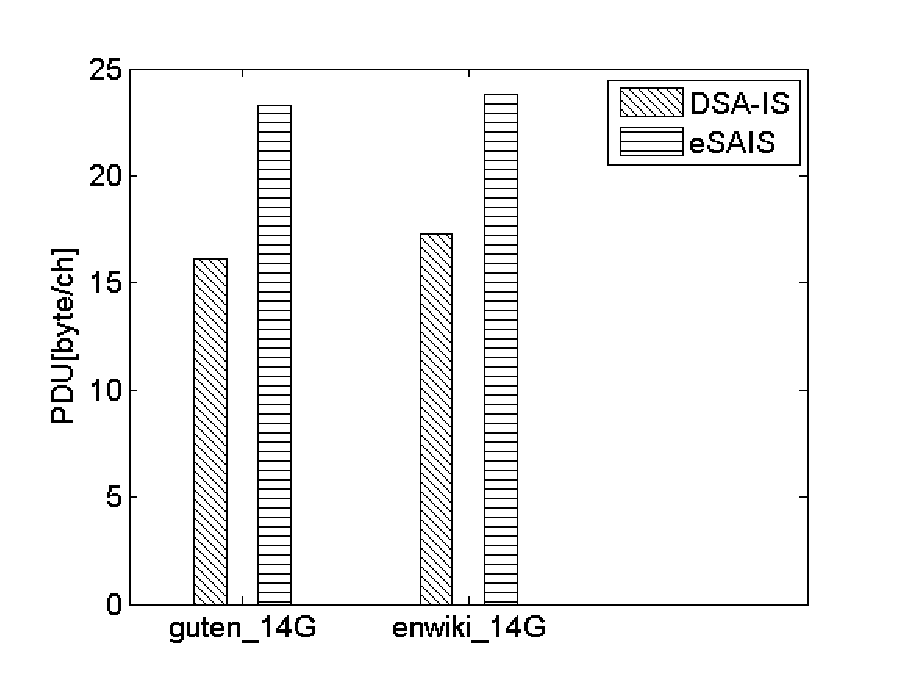
\includegraphics[width = 0.9\columnwidth]{pdu_cmp1}
		}
	\hfil
	\subfigure{
		\label{subfig:iov_cmp1}
		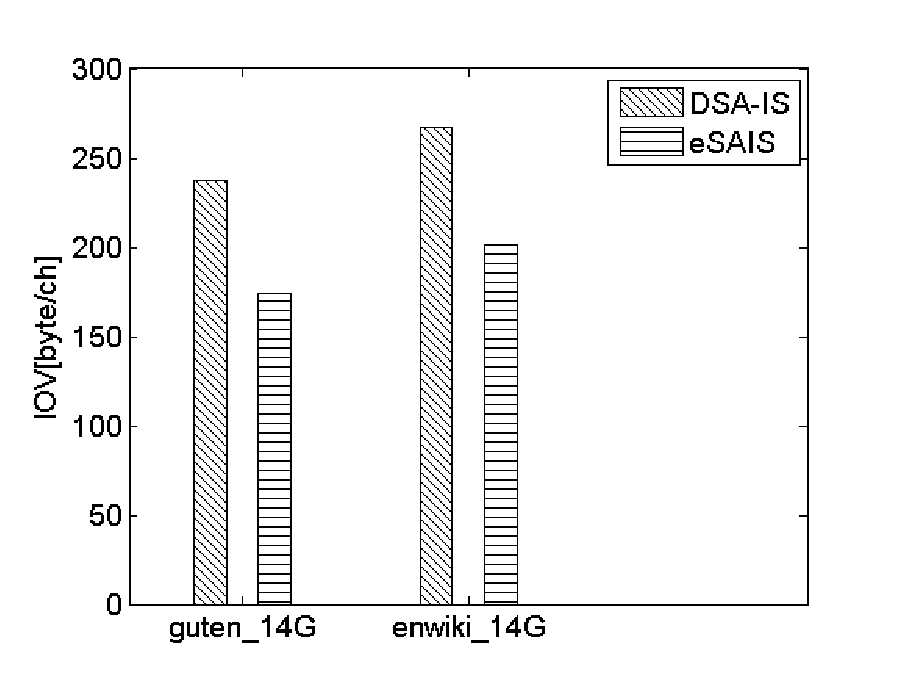
\includegraphics[width = 0.9\columnwidth]{iov_cmp1}
		}
	\hfil
	\subfigure{
		\label{subfig:ct_cmp1}
		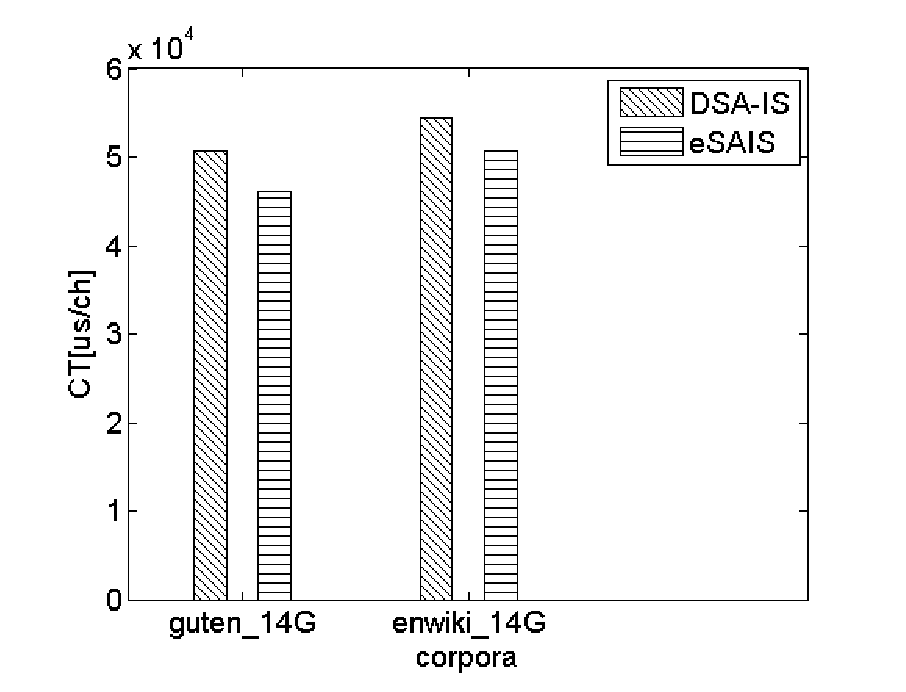
\includegraphics[width = 0.9\columnwidth]{ct_cmp1}
		}
	\caption{Experimental results for DSA-IS and eSAIS on guten\_14G and enwiki\_14G in terms of peak disk usage, I/O volume and construction time.}
	\label{fig:performance_analysis1}
\end{figure}

% Table
\begin{table*}%
\caption{Comparison of Reduction and Induction I/O Volumes Amongst DSA-IS, DSA-IS+ and eSAIS on enwiki}
\label{tbl:volume_cmp}
\centering
\begin{tabular}{|c|c|c|c|c|c|c|c|c|c|c|c|c|}
	\hline
	\multicolumn{1}{|c}{} & \multicolumn{4}{|c|}{eSAIS} & \multicolumn{4}{c|}{DSA-IS} & \multicolumn{4}{c|}{DSA-IS+ ($D_1 = 8$, $D_2 = 10$)}\\\hline
	\hline
	Size & Red. & Ind. & Total & Ratio & Red. & Ind. & Total & Ratio & Red. & Ind. & Total & Ratio\\\hline
	1G & 36.6 & 132.8 & 169.4 & 0.27 & 81.3 & 105.9 & 187.2 & 0.76 & 39.1 & 104.3 & 143.4 & 0.37\\\hline
	2G & 36.0 & 141.9 & 177.9 & 0.25 & 83.5 & 108.2 & 191.7 & 0.77 & 37.8 & 106.4 & 144.2 & 0.35\\\hline
	4G & 35.6 & 152.1 & 187.7 & 0.23 & 94.3 & 118.9 & 213.2 & 0.79 & 42.4 & 117.0 & 159.4 & 0.36\\\hline
	8G & 35.2 & 165.7 & 200.9 & 0.21 & 107.8 & 132.3 & 240.1 & 0.81 & 43.7 & 129.9 & 173.6 & 0.33\\\hline
	14G & 35.0 & 172.1 & 207.1 & 0.20 & 121.9 & 146.6 & 268.5 & 0.83 & 43.8 & 142.3 & 186.1 & 0.30\\\hline
\end{tabular}
\end{table*}%

The above phenomenon can be explained as follows. During the reduction phase, DSA-IS partitions the input string $x$ into multiple blocks and induced sorts the substrings of each block in the internal memory. Then it reuses the induced sorting method to sort all the substrings of $x$ in the external memory by merging the block-wise results residing on disks. In contrast with DSA-IS, eSAIS splits $x$ into fixed-size partitions and sorts the substrings of each partition in the internal memory by calling std::sort. Then, it generates the global result by merging the partial ones with an internal memory heap. This leads to a higher I/O efficiency against DSA-IS.

We attempt to reduce the I/O overhead for DSA-IS by using the substring sorting and naming methods described in Section~\ref{sec:dsais_plus}. Our program for the enhanced algorithm DSA-IS+ introduces two parameters $D_1$ and $D_2$ to respectively specify the threshold value $D$ for classifying the substrings in $x$ and the reduced strings $\{x1, x2, ...\}$ according to the instructions in Section~\ref{subsec:dsais_plus_method_b}. As observed from Table~\ref{tbl:volume_cmp}, the total I/O volumes for DSA-IS+ and eSAIS are similar and the ratio of the reduction and induction I/O volumes for either of them is no more than half of that for DSA-IS. This substantial improvement leads to a great speedup against DSA-IS. Figure~\ref{fig:performance_analysis2} shows the performance trends of DSA-IS+ and eSAIS on guten and enwiki as the corpora size increases from $1G$ to $14G$, which indicates that the speed of DSA-IS+ is similar to that of eSAIS and its peak disk usage remains at a low level as the same as that of DSA-IS.

\begin{figure*}[htbp]
\centering
\subfigure[guten]{
	\begin{minipage}[b]{0.45\textwidth}
		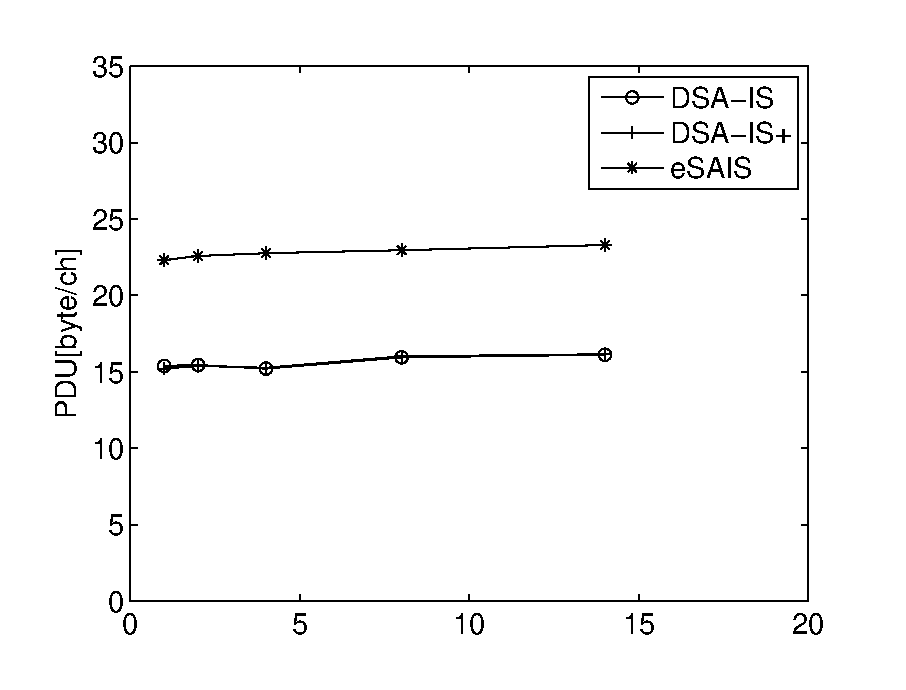
\includegraphics[width=1\textwidth]{pdu_cmp2_guten} \\
		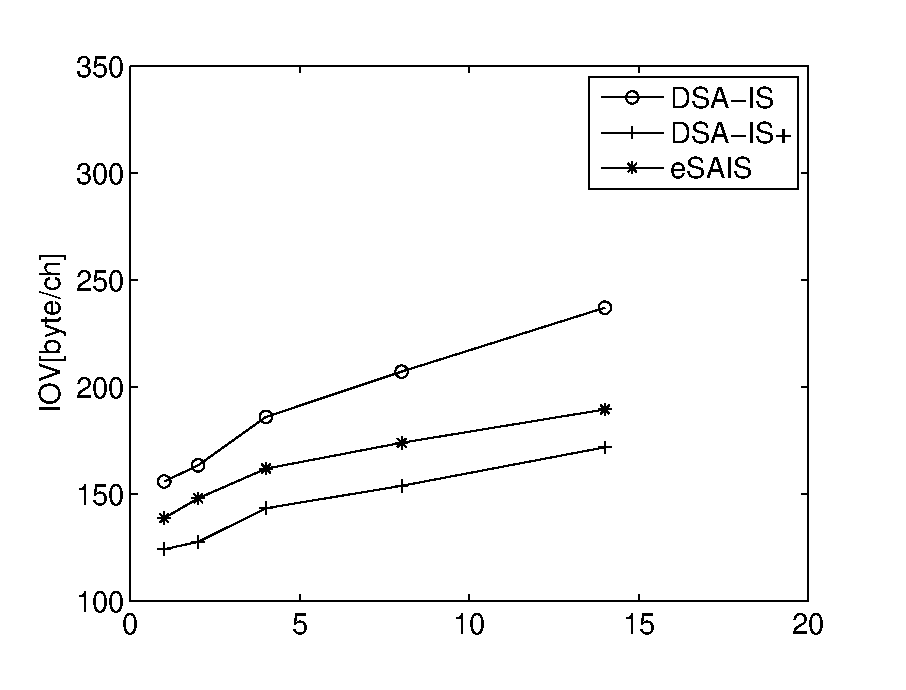
\includegraphics[width=1\textwidth]{iov_cmp2_guten} \\
		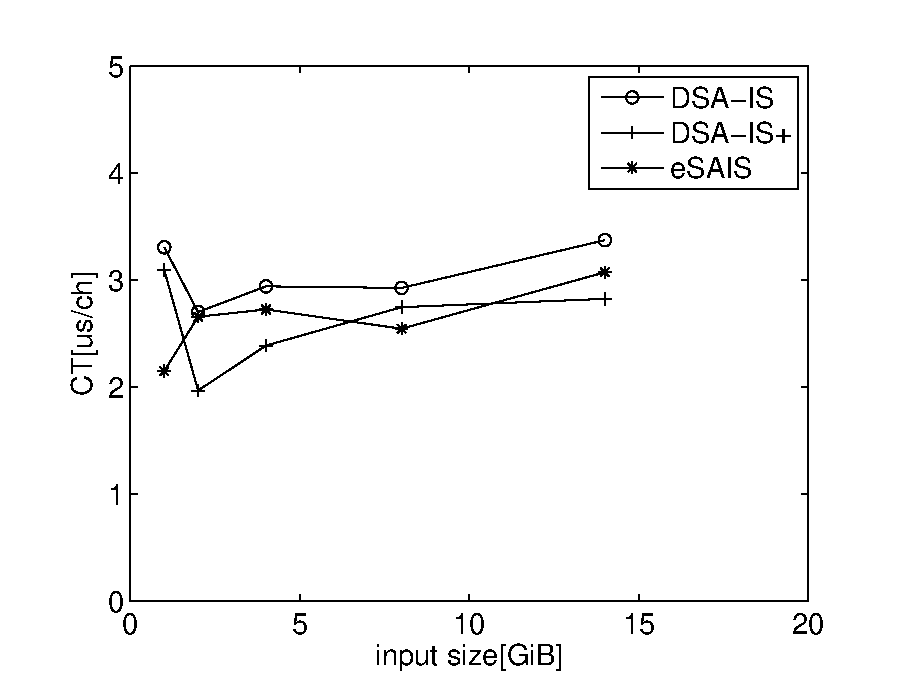
\includegraphics[width=1\textwidth]{ct_cmp2_guten}
	\end{minipage}
}
\subfigure[enwiki]{
	\begin{minipage}[b]{0.45\textwidth}
		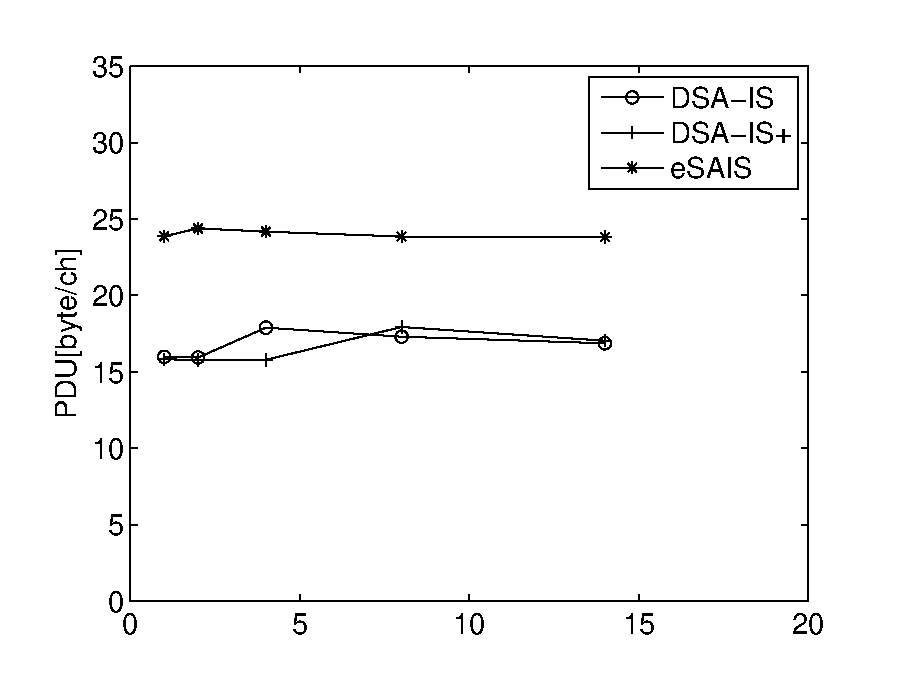
\includegraphics[width=1\textwidth]{pdu_cmp2_enwiki} \\
		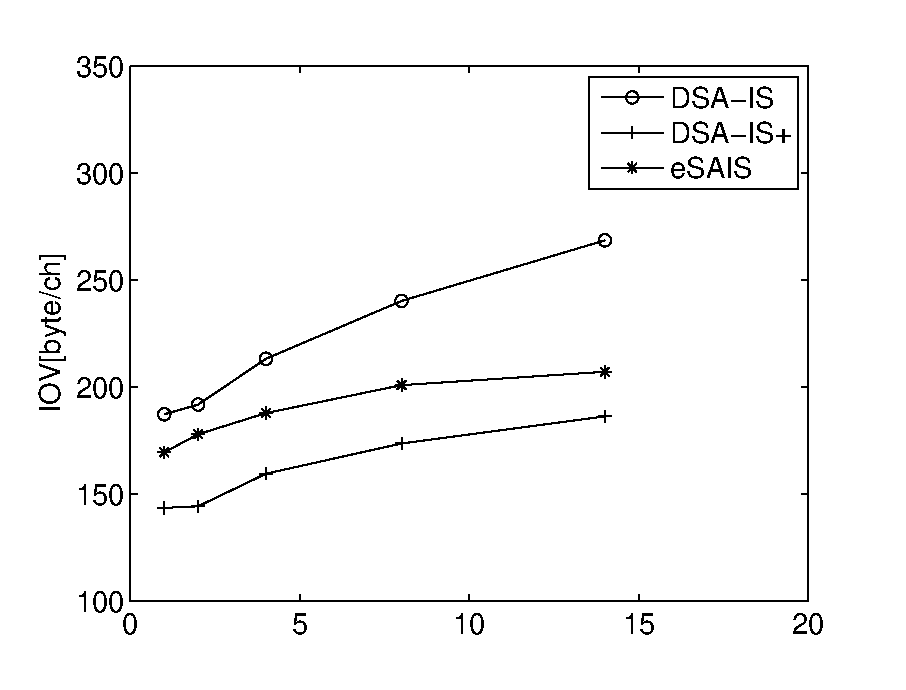
\includegraphics[width=1\textwidth]{iov_cmp2_enwiki} \\
		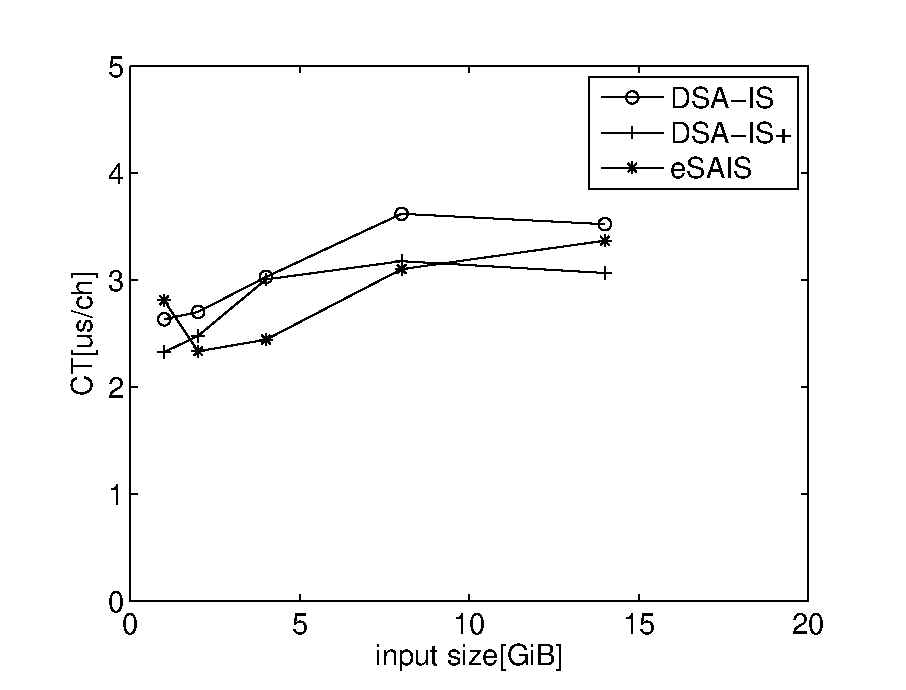
\includegraphics[width=1\textwidth]{ct_cmp2_enwiki}
	\end{minipage}
}
\caption{Experimental results for DSA-IS, DSA-IS+ and eSAIS on guten and enwiki in terms of peak disk usage, I/O volume and construction time, where $D_1 = 8$, $D_2 = 10$ and the input size varies in \{1, 2, 4, 8, 14\} GiB. }
\label{fig:performance_analysis2}
\end{figure*}

%As with other external memory suffix sorting algorithms, DSA-IS+ is I/O-intensive and its construction speed is presumed to be linearly proportional to the I/O volume. However, our experiments indicate that the ratio of the reduction and induction time is much higher than that of the reduction and induction volume. This phenomenon is possibly due to the performance of the STXXL library. For implementation simplicity, we organize the item of DSAITEM arrays by using the sorter and priority queue containers provided by STXXL in our programs. This

A series of experiments are conducted to investigate the effect of $D_1$ and $D_2$ on the performance of DSA-IS+. As shown in Figure~\ref{fig:performance_analysis3}, the time consumption of DSA-IS+ gets smaller as $D_2$ becomes larger, while the peak disk usage and I/O volume are almost unchanged. Furthermore, the data of Table~\ref{tbl:effect_of_D} indicates that a small variation on the values of $D_1$ and $D_2$ can incur a significant fluctuation on the speed of DSA-IS+. For instance, when changing $(D_1, D_2)$ from $(8, 10)$ to $(16, 16)$, the construction time for the uniprot dataset decreases from 2.64 to 2.24 microseconds per character. This is because the proportions of long LMS substrings of $x$ and $\{x1, x2,...\}$ decrease when $D_1$ and $D_2$ increase. Recall that, after partitioning $x$ into blocks, DSA-IS+ sorts the long LMS substrings of each block in RAM and merges them by an external memory sorter, which is time-consuming when the number of long LMS substrings is large. In our program, the ratio of long and short LMS substrings can be controlled by adjusting the values of $D_1$ and $D_2$. However, when $D_1$ and $D_2$ get larger, the min heap also takes more time to merge the sorted short and long LMS substrings, as each string comparison takes $\mathcal{O}(D_1)$ and $\mathcal{O}(D_2)$ time in the first and recursion levels, respectively. Fortunately, Table~\ref{tbl:long_short_distribution} shows that the majority of LMS substrings in real datasets are considerably short. In practice, we can set $D_1$ and $D_2$ according to the statistics of the length distribution of LMS substrings, where the statistics can be collected when partitioning $x$ at the beginning of the reduction phase.

\begin{table*}[htbp]
\caption{Effects of $D_1$ and $D_2$ for DSA-IS+}
\label{tbl:effect_of_D}
\centering
\begin{tabular}{|c|c|c|c|c|c|c|c|c||c|c|c|c|c|}
	\hline
	\multicolumn{1}{|c}{} & \multicolumn{3}{|c}{eSAIS} & \multicolumn{10}{|c|}{DSA-IS+}\\\hline
	\hline
	Corpora & PDU & IOV & CT & $D_1$ & $D_2$ & PDU & IOV & CT  & $D_1$ & $D_2$ & PDU & IOV & CT\\\hline
	uniprot & 22.71 & 162.01 & 2.50 & 8 & 10 & 14.27 & 146.10 & 2.64 & 16 & 16 & 14.27 & 144.90 & 2.24 \\\hline
	proteins & 24.09 & 172.29 & 2.33 & 8 & 10 & 16.12 & 147.92 & 2.28 & 20 & 12 & 16.12 & 147.85 & 2.14 \\\hline
	genome & 22.64 & 157.41 & 2.15 & 8 & 10 & 15.34 & 142.05 & 2.75 & 20 & 12 & 15.34 & 140.89 & 2.25 \\\hline
\end{tabular}
\end{table*}%

\begin{figure}[htbp]
	\centering
	\subfigure{
		\centering
		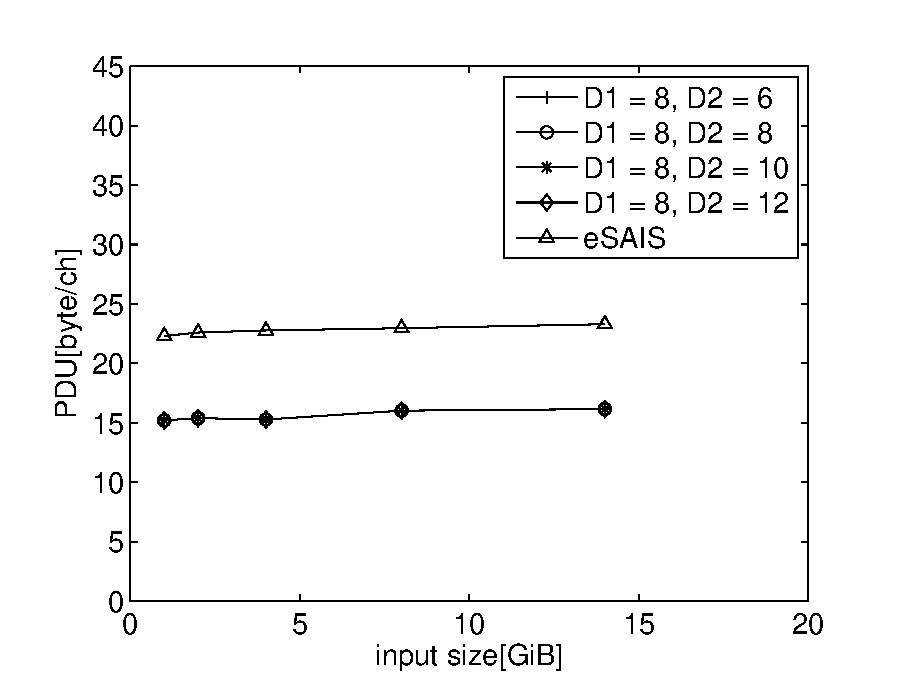
\includegraphics[width=0.9\columnwidth]{pdu_cmp3}
		\label{subfig:pdu_cmp3}
	}
	\hfil
	\subfigure{
		\centering
		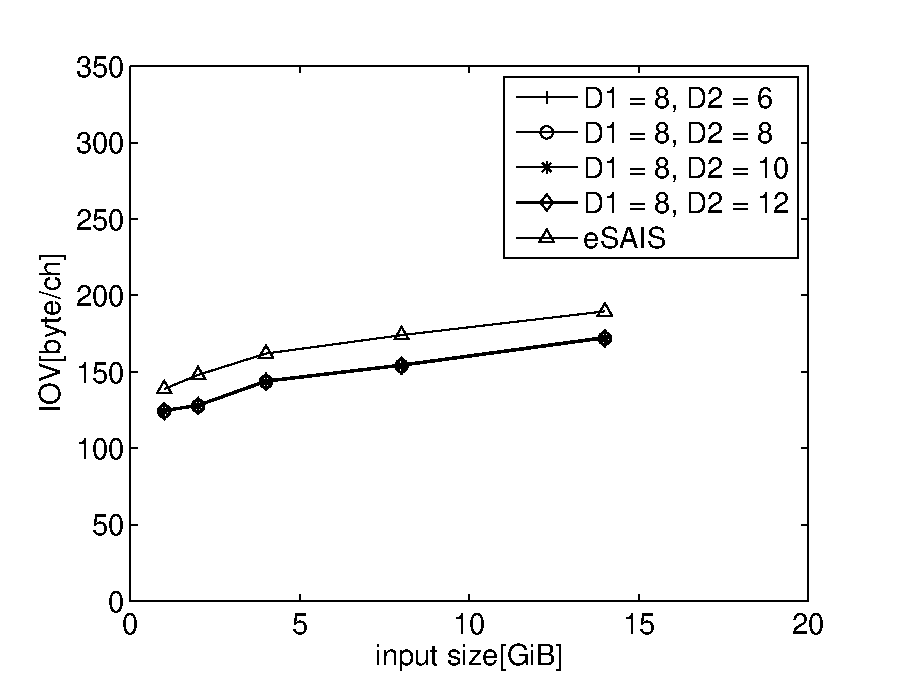
\includegraphics[width=0.9\columnwidth]{iov_cmp3}
		\label{subfig:iov_cmp3}
	}
	\hfil
	\subfigure{
		\centering
		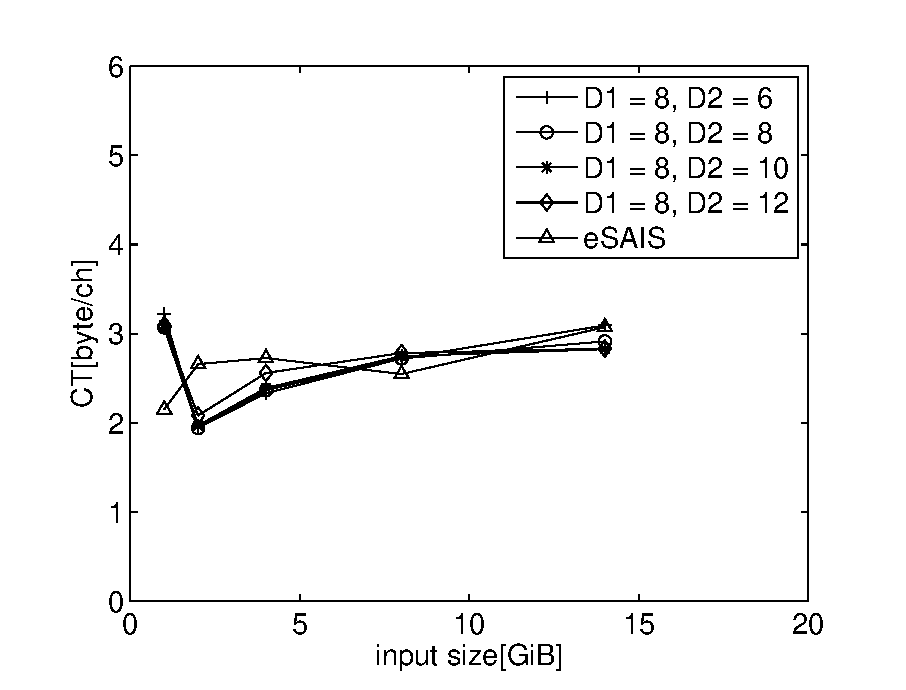
\includegraphics[width=0.9\columnwidth]{ct_cmp3}
		\label{subfig:ct_cmp3}
	}
	\caption{Experimental results for DSA-IS+ and eSAIS on guten in terms of peak disk usage, I/O volume and construction time, where $D_1 = 8$, $D_2$ ranges in \{6, 8, 10, 12\} and the input size varies in \{1, 2, 4, 8, 14\} GiB. }
	\label{fig:performance_analysis3}
\end{figure}


\begin{table*}[htbp]
\caption{Statistics on the Length Distribution of Long and Short LMS Substrings for DSA-IS+}
\label{tbl:long_short_distribution}	
\centering
\begin{tabular}{|c|c|c|c|c|c|c|c|c|c|c|}
	\hline
	\multicolumn{11}{|c|}{level 0} \\\hline
	Corpora & $D_1$ & long & short & total & ratio & $D_1$ & long & short & total & ratio\\\hline
	uniprot & 8 & 30243605 & 785997413 & 816241018 & 0.963 & 16 & 3850755 & 812390263 & 816241018 & 0.999\\\hline
	proteins & 8 & 1687673 & 377404329 & 379092002 & 0.999 & 20 & 10930 & 379081072 & 379092002 & 0.999\\\hline
	genome & 8 & 19446841 & 773670266 & 793117107 & 0.975 & 20 & 509998 & 792607109 & 793117107 & 0.999\\\hline
	\multicolumn{11}{|c|}{level 1}\\\hline
	Corpora & $D_2$ & long & short & total & ratio & $D_2$ & long & short & total & ratio\\\hline
	uniprot & 10 & 11849 & 263748775 & 263760624 & 0.995 & 16 & 380 & 263760244 & 263760624 & 0.999\\\hline
	proteins & 10 & 18126 & 123772731 & 123790857 & 0.996 & 20 & 2937 & 123787920 & 123790857 & 0.999\\\hline
	genome & 10 & 311607 & 248243216 & 248554823 & 0.999 & 20 & 153845 & 248400978 & 248554823 & 0.999\\\hline
\end{tabular}
\end{table*}%


\subsection{Performance Evaluation on Checking Methods}

\begin{table*}[htbp]
	\caption{Overall Performance of DSA-IS+ and eSAIS with CM1 and CM2 on enwiki\_8G}
	\label{tbl:check_overhead}
	\centering
	\begin{tabular}{|c|c|c|c|c|c|c|}
		\hline
		& \multicolumn{3}{|c|}{DSA-IS+ ($D_1 = 8$, $D_2 = 10$)} & \multicolumn{3}{c|}{eSAIS}\\\hline
		Checking Method & PDU & IOV & CT & PDU & IOV & CT \\\hline
		CM1 & 17.93  & 180.01 & 3.10 & - & - & - \\\hline
		CM2 & 26.00 & 231.68 & 4.00 & 27.00 & 246.93 & 3.74 \\\hline
		no check & 17.93  & 173.67	& 3.17 & 23.85 & 200.93 & 3.10 \\\hline
	\end{tabular}
\end{table*}%


We make a performance comparison of the proposed checking method and the work presented in~\cite{Karkkainen2003}, which are denoted by CM1 and CM2, respectively. For performance evaluation, we integrate CM1 into the program of DSA-IS+ following Section~\ref{subsec:sachecker:implementation} and reuse the implementation for CM2 in the program of eSAIS to verify the outputs of DSA-IS+ and eSAIS. Table~\ref{tbl:check_overhead} gives a glimpse of the performance overhead for the two checking methods. It can be seen that, when checking the suffix array of enwiki\_8G by using CM2, both time and I/O volume for verification are about one-fifth of that for construction. On the other hand, CM1 has almost no negative impact on the overall performance. As demonstrated in lines 3 and 5, the peak disk usage for CM1 is no more than that for DSA-IS+ and the increase in the I/O volume can be ignored. It worth mentioning that the data of the running time for the combination of DSA-IS+ and CM1 is a bit shorter than that for the plain DSA-IS+. This is a normal phenomenon due to the fluctuating I/O performance, which in turn indicates that the time overhead consumed by CM1 is also negligible.


	

\section{Conclusion} \label{sec:conclusion}

For better performance, we redesign the reduction phase of DSA-IS by employing two methods for sorting and naming substrings. The program of the enhanced algorithm DSA-IS+ is engineered by the STXXL library to achieve a high I/O efficiency. Our experiments indicate that DSA-IS+ requires only around $16/24=0.67$ peak disk usage as that for eSAIS and runs as fast as the latter on various real datasets.

We describe an SA checker of linear time and space complexities that can be used to verify a suffix array during the time when it is being built. In combination with DSA-IS+, our checking method almost has no influence on the overall performance and is more efficient than the existing work in terms of time, space and I/O efficiencies.

% Bibliography
\bibliographystyle{IEEEtran}
\bibliography{IEEEabrv,bibfile}
	
\end{document}


